\documentclass[a4paper,12pt]{article}
\usepackage{fullpage}
\usepackage{setspace}
\usepackage[utf8]{inputenc}
\usepackage[T1]{fontenc}
\usepackage[french]{babel}
\usepackage[final]{pdfpages}
\usepackage{graphicx}
\usepackage{pgfgantt}
\usepackage[colorlinks=true,linkcolor=black]{hyperref}
\usepackage{microtype}
\DisableLigatures[<,>]{encoding=T1,family=tt*}
\begin{document}
% PAGE DE GARDE
	\begin{flushright}
		
\includegraphics[scale=0.3]{UGA.eps}
	\end{flushright}
	\vspace{1.5cm}
	\begin{center}
		{\Large Universit\'e{} Joseph Fourier\\
		D\'e{}partement Licence Sciences \& Technologie}
		\vspace{1cm}
		{\Huge RAPPORT DE STAGE}\\
		\vspace{3mm}
		{\Large Calcul parall\`ele sur GPU}\\
		\vspace{2mm}
		Picard Micha\"el\\
		6 juin 2016 - 1er juillet 2016\\
		\vspace{4mm}
		\includegraphics[scale=0.3]{LIG.eps}
		\includegraphics[scale=0.3]{INRIA.eps}
	\end{center}
	\vspace{1cm}
	\begin{flushleft}
		Laboratoire d'acceuil : LIG - INRIA\\
		\'E{}quipe : Polaris\\
		Directeur du laboratoire : GAUSSIER Eric (LIG)\\
		\hspace{4.65cm} GROS Patrick (INRIA)\\
		Responsable du stage : HUARD Guillaume
	\end{flushleft}
	\vspace{8mm}
	\begin{flushright}
	License MIN - 1\`ere ann\'e{}e\\
	Ann\'e{}e universitaire : 2015 - 2016
	\end{flushright}
	
	\newpage
	{\scriptsize Cette page a \'e{}t\'e{} laiss\'e{} intentionnellement blanche.
	\newpage
%SOMMAIRE
	\renewcommand{\contentsname}{
		\begin{center}
			Sommaire
		\end{center}
	}
	\setcounter{tocdepth}{3}
	\tableofcontents
% CORPS DU RAPPORTS
	\newpage
	\section{Remerciement}
		\indent Je tiens à remercier Mr HUARD Guillaume pour son accueil au sein de l'équipe Polaris, pour sa gentillesse et pour le temps qu'il m'a accord\'e{} pour m'expliquer de nouvelles notions, tant utilitaire, m\'e{}thodique qu'algorithmique, pour ses encouragements et son soutien durant ce stage, qui m'a permis de d\'e{}couvrir le m\'e{}tier d'enseignant-chercheur. \\
		\indent Je remercie aussi Mr BENIAMINE David, actuellement en th\`ese à l'INRIA, pour le temps pass\'e{} à m’accueillir sur les locaux et ses conseils utiles pour me permettre d'avancer durant le stage.\\
		\indent Je remercie Mme SIMON Annie, l'assistante de l'\'e{}quipe Polaris pour son temps sur mon dossier, et pour m'avoir aid\'e{} à r\'e{}gler les nombreux impr\'e{}vus à propos des conventions de stages et autres formalit\'e{}s.\\
		\indent Je remercie aussi l'INRIA et le LIG ainsi que leur directeur, Mrs GAUSSIER Eric et GROS Patrick, pour m'avoir permis de participer à une pr\'e{}sentation d'algorithmie à des lycéens, dans leur locaux de Montbonnot, sous la tutelle de Mr HUARD.\\
		\indent Je remercie enfin l'UGA, le DLST et Mmes MANDON Nina, COGNE Lydie, DARRACQ Marie-Cécile et CAJOT Patricia pour m'avoir donné l'opportunité de participé à ce stage.
	\newpage
	\section{Introduction}
	\indent Mon stage à l'Inria portant sur le Calcul parrallèle sur GPU, j'ai été amené à utilisé de nombreux outils.\\
	\noindent Je vais donc vous présenter en premier lieu la structure d'accueil du stage, puis je vous parlerai des différents outils utilisée durant ce stage, avant de vous présenter mon évolution durant mes 4 semaines en tant que stagiaire.
	\subsection{Environnement d'acceuil : INRIA \& LIG}
	\indent L’INRIA est un centre de recherche cr\'e{}e \`a sous le r\'e{}gime du Général DeGaule et compte aujourd’hui presque une dizaine de centres en France. Le centre Rhône-Alpes a été crée en 1992.\\
	\indent \`A Grenoble le directeur du centre est Mr GROS Patrick depuis le 1er Décembre 2014. La plupart des \'e{}quipes-projets Inria grenobloises sont des
\'e{}quipes communes avec le CNRS, l’université Joseph Fourier, et Grenoble INP au sein des laboratoires :
\begin{itemize}
\item Laboratoire d’informatique de Grenoble (LIG)
\item Laboratoire Jean Kuntzmann (LJK)
\item Laboratoire Grenoble Images Parole Signal Automatique (GIPSA)
\item Laboratoire Adaptation et Pathogénie des Microorganismes (LAPM)
\end{itemize}
	\indent \indent L'\'e{}quipe qui m'a accueilli est l'\'e{}quipe POLARIS, appartenant au LIG, et nouvellement install\'e{}e au bat\^iment IMAG sur le campus universitaire de Grenoble. Le responsable du LIG est Mr GAUSSIER Eric, tandis que le responsable de l'\'e{}quipe POLARIS est Mr Legrand Arnaud. Le thème de recherche de cette \'e{}quipe est << Calcul distribu\'e et \`a haute performance~ >>, plus pr\'e{}cis\'e{}ment << Performance analysis and optimization of LARge Infrastructures and Systems >>.
	\subsection{Outils et Méthodes utilis\'e{}s}
	\subsubsection{CUDA et les cartes graphiques NVIDIA}
	\subsubsection{GIT}
	\subsubsection{Abstraction, g\'e{}n\'e{}ralisation et factorisation du code}
	\subsubsection{R et Rmarkdown}
	\subsubsection{\LaTeX}
	\subsection{Pourquoi ce stage?}
	\newpage
	\section{Mon parcours}
	\newpage
	\section{Conclusion}
	\begin{ganttchart}{1}{23}
		\def\mavar#1{%
			\ifcase #1 6\or 7\or 8\or 9\or 10\or 13\or 14\or 15\or 16\or 17\or 20\or 21\or 22\or 23\or 24\or 27\or 28\or 29\or 30\or 1\fi%
		}
		\gantttitle{Juin}{19}
		\gantttitle{Juillet}{4}\\
		\gantttitlelist[
			title list options=%
			{var=\y, evaluate=\y as \x%
			using "\mavar{\y}"}]{0,...,18}{1}
		\gantttitlelist[
			title list options=%
			{var=\y, evaluate=\y as \x%
			using "\mavar{\y}"}]{19}{4}\\
		\ganttbar{CUDA}{1}{5}\\
		\ganttbar{D\'e{}veloppement}{6}{14}\\
		\ganttbar{GIT}{3}{5}\\
		\ganttbar{R}{6}{8}
		\ganttbar{R}{13}{18}\\
		\ganttbar{\LaTeX}{18}{20}
		\path[->,>=latex] (elem0.east) edge[out=0,in=180] (elem1.west);
	\end{ganttchart}
%ANNEXES

	\newpage
	\vspace*{\stretch{1}}
	\begin{center}
		\section*{Annexe : Rapport d'exp\'e{}rience}
		\addcontentsline{toc}{section}{Annexe : Rapport d'exp\'e{}rience}
	\end{center}
	\vspace*{\stretch{1}}
%Inclusion du pdf de notre rapport de projet
	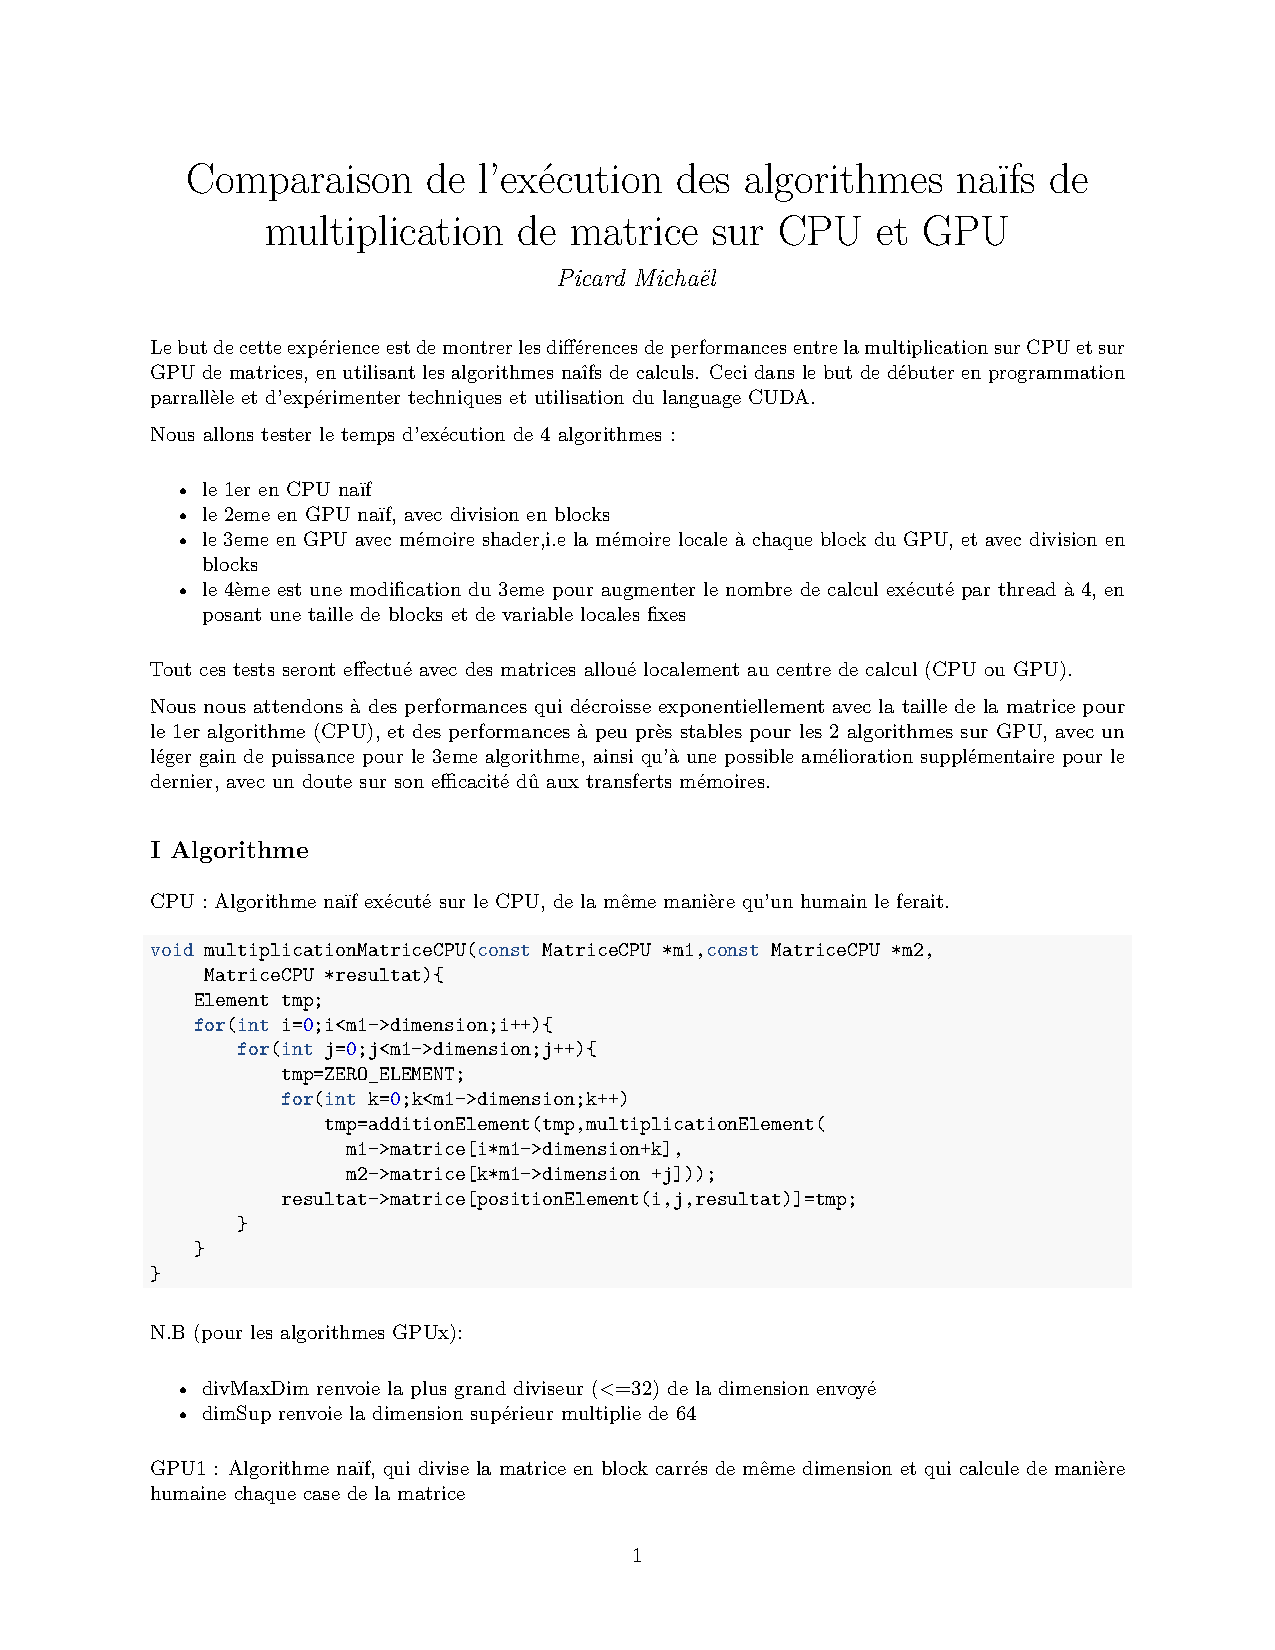
\includepdf[pages=-]{analyse.pdf}
\end{document}